\documentclass{beamer}

\usetheme[plain]{NTU}
\usepackage[]{media9}

\usepackage[absolute,overlay]{textpos}
\usepackage{tikz}
\usepackage[english]{babel}
\usepackage[latin1]{inputenc}
\usepackage{times}
\usepackage[T1]{fontenc}
\usepackage{tikz} % For drawing diagrams
\usetikzlibrary{shapes,arrows,positioning,automata,fit}
% Or whatever. Note that the encoding and the font should match. If T1
% does not look nice, try deleting the line with the fontenc.


\usepackage{ragged2e}


\newcommand<>{\PutAt}[3][0pt]{%
    {\only#4{\begin{textblock*}{#1}#2%
      #3
    \end{textblock*}}}%
}

\newcommand{\ShowPutAtGrid}{
    \begin{textblock*}{128mm}(0cm,0cm)
    \tikz[color=red!20!white]\draw[very thin, step=5mm] (0mm,0mm) grid (130mm,100mm);
    \end{textblock*}
    \begin{textblock*}{128mm}(0cm,0cm)
    
\begin{tikzpicture}[color=red]
      \draw[step=1cm] (0,0mm) grid (130mm,100mm);   
      \foreach \n in {0,...,12}
        \draw[xshift=.5mm,yshift=-1.5mm, inner sep=0pt, anchor=west] (\n,10) node {\scriptsize{\textbf{\n}}};
      \foreach \n in {1,...,9}
        \draw[xshift=.5mm,yshift=-1.5mm, inner sep=0pt, anchor=west] (0,10-\n) node {\scriptsize{\textbf{\n}}};
    \end{tikzpicture}
    \end{textblock*}
}

\newcommand<>{\NormalBox}[2][]{%
  \only#3{\tikz[#1, every node/.style={shape=rectangle,draw,fill=white, #1}]\node []{#2};}
}

\setbeamercolor{blue}{fg=blue!50!black}
\setbeamercolor{red}{fg=red!80!black}
\setbeamercolor{magenta}{fg=brown!50!red!60!black}

\newcommand{\blue}{blue!50!black} 
\newcommand{\red}{red!80!black} 
\newcommand{\green}{yellow!95!black} 
\newcommand{\magenta}{brown!50!red!60!black}

\newcommand*\oldmacro{}%
\let\oldmacro\insertshorttitle%
\renewcommand*\insertshorttitle{%
  \oldmacro\hfill%
  \insertframenumber\,/\,\inserttotalframenumber}





\definecolor{shadecolor}{RGB}{255,255,224}
\newcommand{\mybox}[1]{\par\noindent\colorbox{shadecolor}
{\parbox{\dimexpr\textwidth-10\fboxsep\relax}{#1}}}

\usepackage{xcolor}


\title[]{Assured Machine Learning} % The short title appears at the bottom of every slide, the full title is only on the title page

%\subtitle
\author[]{Xiaozhe Gu, Arvind Easwaran}
\institute[NTU]{School of Computer Science and Engineering \\ Energy Research Institute (ERI@N) \\ \vspace{2mm} Nanyang Technological University, Singapore}



\date[June, 2018]{June, 2018}



% Delete this, if you do not want the table of contents to pop up at
% the beginning of each subsection:
\AtBeginSection[]
{
  \begin{frame}<beamer>{Outline}
    \tableofcontents[currentsection]
 \end{frame}
}


% If you wish to uncover everything in a step-wise fashion, uncomment
% the following command: 

% \beamerdefaultoverlayspecification{<+->}

% \setbeameroption{show notes on second screen=left}

\begin{document}

\begin{frame}
  \titlepage
\end{frame}

\begin{frame}{Outline}
  \tableofcontents
  % You might wish to add the option [pausesections]
\end{frame}

\section{Motivation}




\begin{frame}[t]{Machine Learning  Applications in Safety-Critical Environments}
Machine learning algorithms are increasingly influencing our lives, and moving into \colorbox{blue!30}{safety-critical} applications.

\begin{columns}[T]
\begin{column}[t]{.35\textwidth}
\color{red}\rule{\linewidth}{2pt}

\begin{itemize}
\only<1>{
  \item Decision making in life-threatening conditions, e.g.,  ML based medical decision support systems.}
  \only<2>{
  \item  Autonomous Robots, e.g., surgical robots, rescue robots, industrial robots, etc.}
  \only<3>{
    \item Self-Driving Vehicles, e.g, autonomous shuttle.
}
  \only<4,5>{
    \item Autonomous Weapons
    \begin{figure}[h]
    \centering
    \caption{SGR-A1 (Source: wikipedia)}
    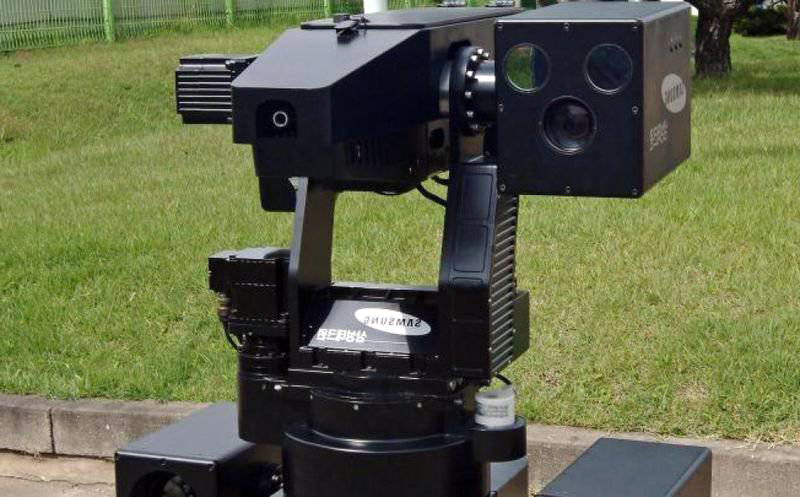
\includegraphics[scale=0.1]{image/SGR.jpg} 
    \end{figure}
% \tiny{wikipedia.org:SGR-A1}
% https://en.wikipedia.org/wiki/SGR-A1
}
\end{itemize}

\end{column}%
% \hfill%


\begin{column}[t]{.6\textwidth}

\color{blue}\rule{\linewidth}{2pt}

\only<1>{
\begin{figure}[h]
\centering
\caption{ML Based Brain Disease Diagnosis\cite{health}}
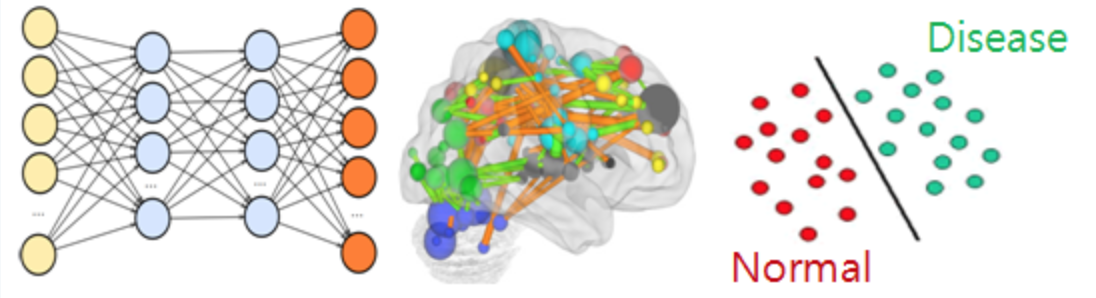
\includegraphics[scale=0.3]{image/medical.png} 
\end{figure}
}


\only<2>{
 \begin{figure}[h]
\centering
\caption{Surgical Robots\cite{surgery}}
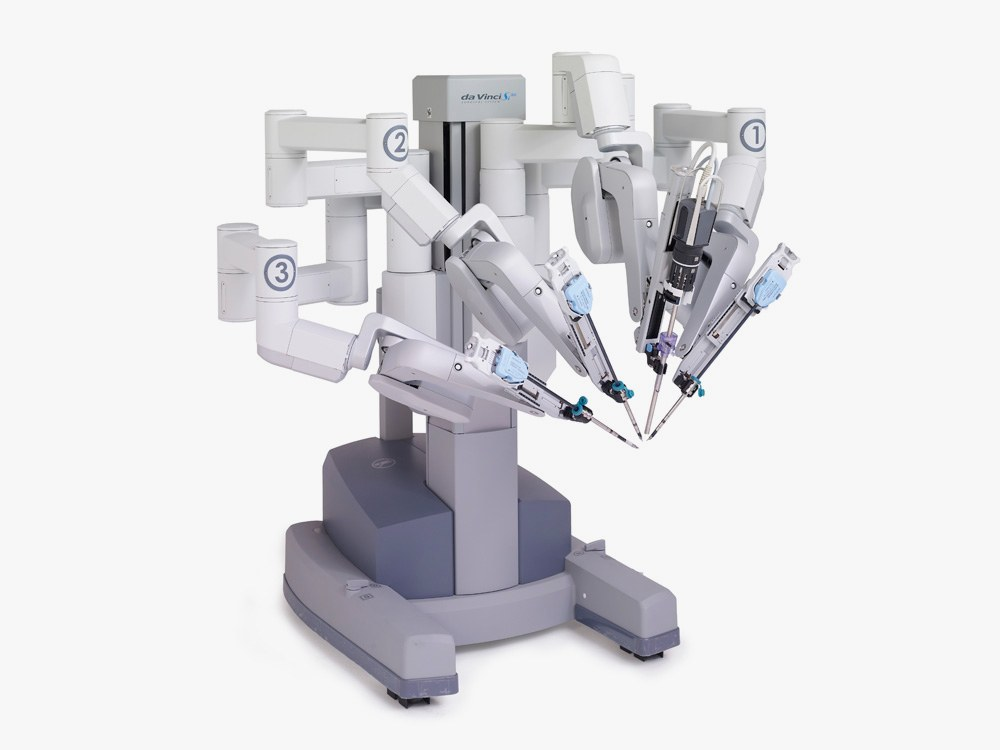
\includegraphics[scale=0.1]{image/surgical.jpg} 
\end{figure}
}

\only<3>{
\begin{figure}[h]
\centering
\caption{Autonomous Shuttle}
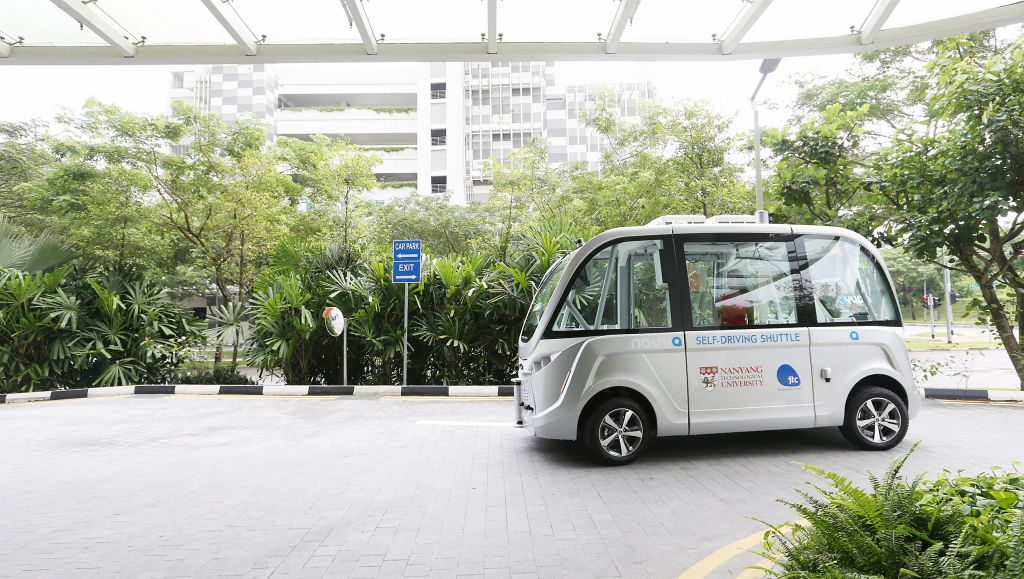
\includegraphics[scale=0.15]{image/car.jpeg} 
\end{figure}
}

\only<5>{
\begin{figure}[h]
\centering
\caption{Source: keelvar.com}
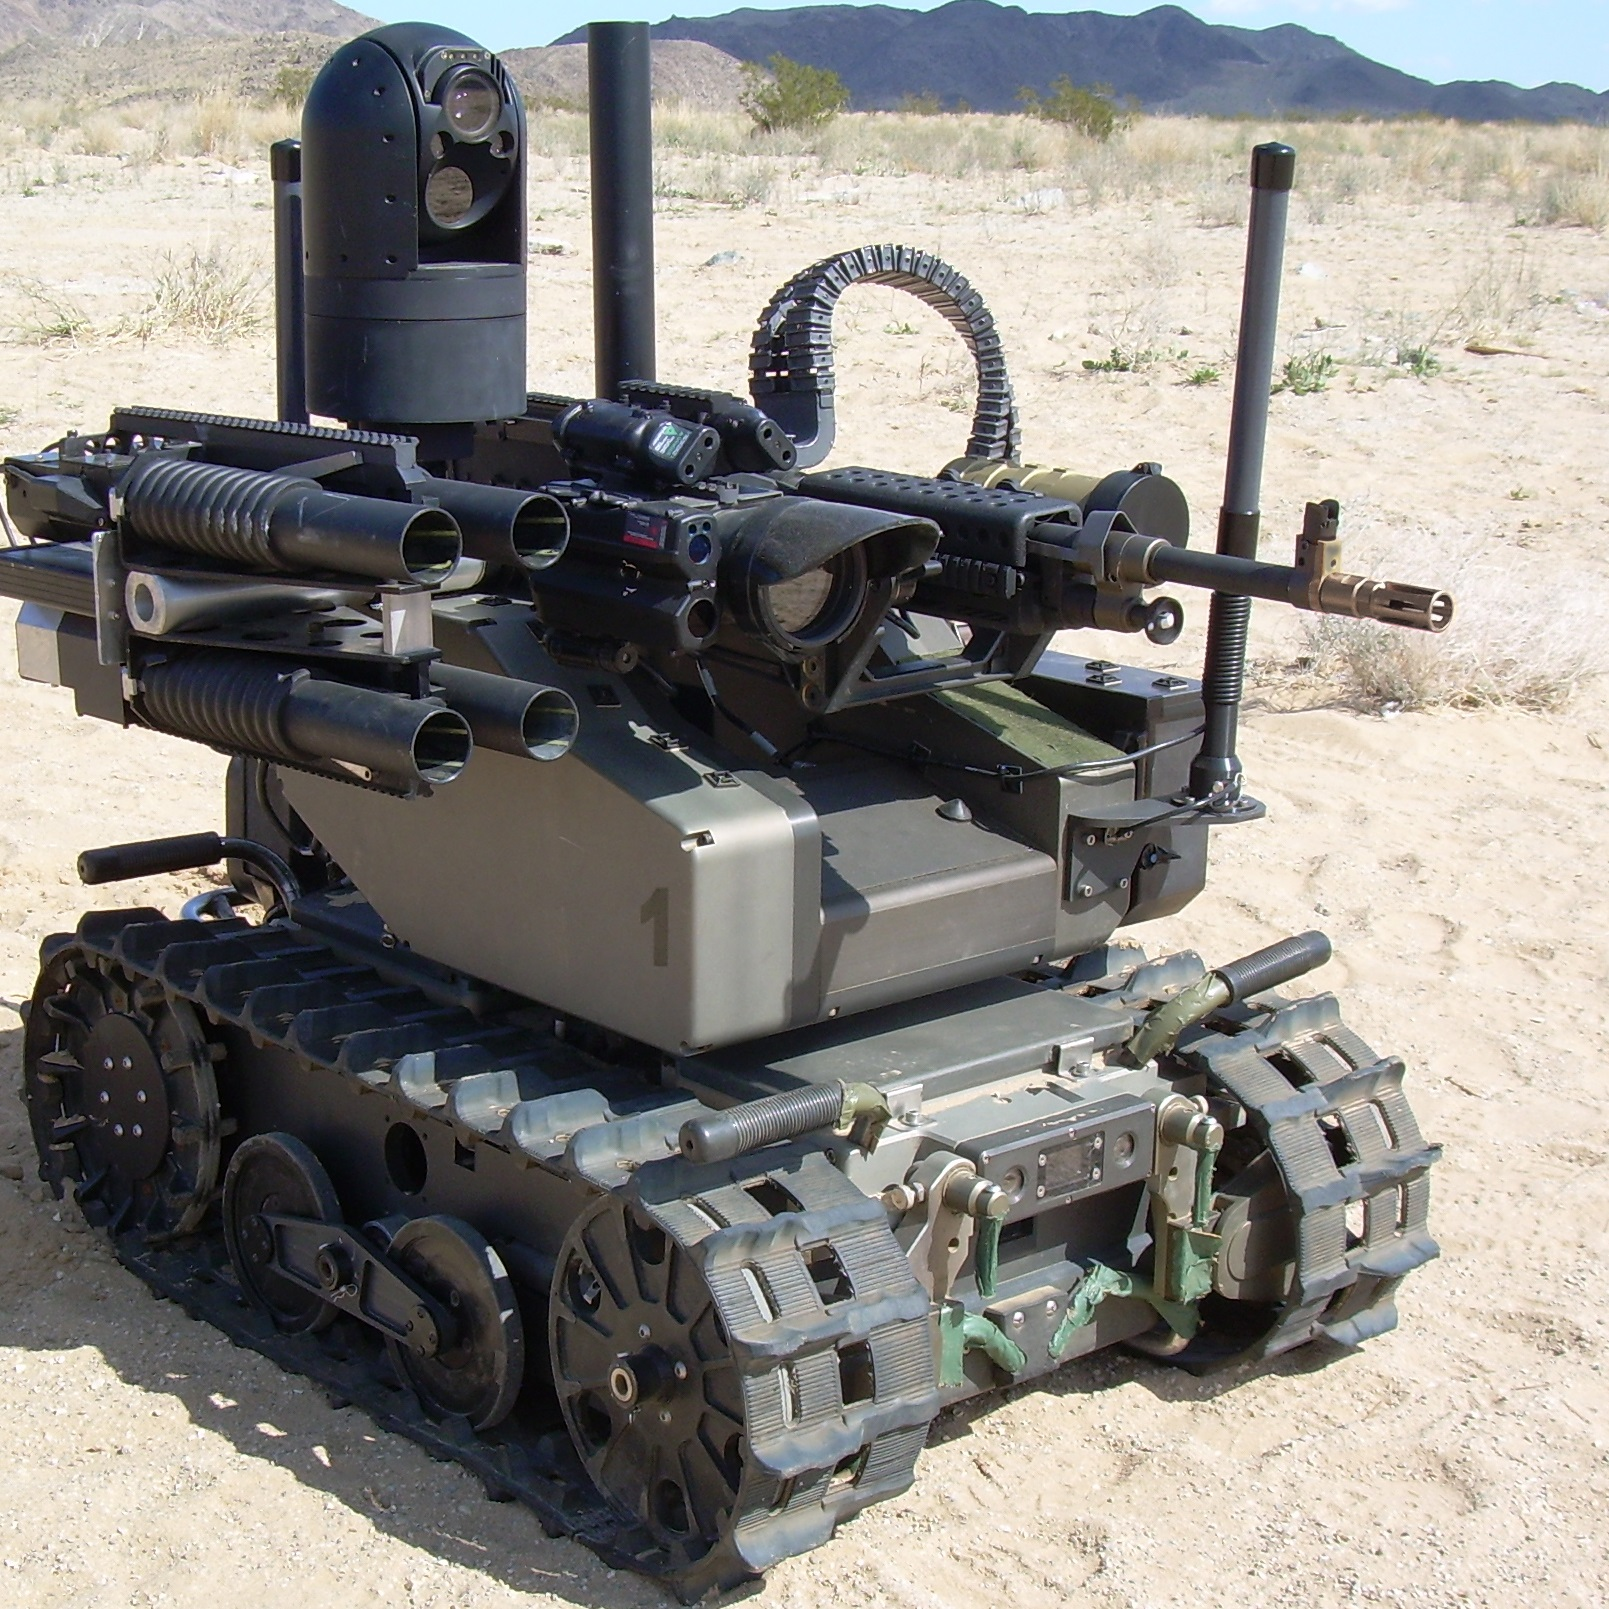
\includegraphics[scale=0.2]{image/MAARS.jpg} 
\end{figure}
% \color{black}\tiny{keelvar.com
% https://keelvar.com/2017/08/21/keelvar-signs-open-letter-autonomous-weapons-delivered-united-nations/}
% }
}

\end{column}%
\end{columns}

  
\end{frame}




\begin{frame}[t]{Traditional Programing versus Machine Learning}

\begin{columns}[T] % align columns
\begin{column}[t]{.5\textwidth}
\color{red}\rule{\linewidth}{2pt}\color{black}
\begin{figure}[h]
\centering
\caption{Traditional Programming}
\includegraphics[scale=0.5]{image/traditionalprogram} 
\end{figure}
\justifying

Traditional programming involves static program instructions  \colorbox{blue!30}{strictly specifying} what we need the computer to do. 
\end{column}
\hfill%

\begin{column}[t]{.5\textwidth}
\vspace{-5mm}

\color{blue}\rule{\linewidth}{2pt} \color{black}
\vspace{-5mm}
\visible<2>{
\begin{figure}[h]
\centering
\caption{Machine Learning}
\includegraphics[scale=0.5]{image/mlprogram} 
\end{figure}
\justifying
ML is a technique that enables computers to learn autonomously and to improve from experience  \colorbox{blue!30}{without being explicitly} \colorbox{blue!30}{ programmed}
}

\end{column}%
\end{columns}


  
\end{frame}


\begin{frame}[t]{Machine Learning Safety}
\visible<1,2>{
\color{black}\rule{\linewidth}{2pt}
Amodei et al.~\cite{Amodei} refer to ML safety as  \emph{`` mitigating  risk in the context of \colorbox{blue!30}{unintended or harmful behaviour} that may emerge from machine learning systems when we  ''
\begin{itemize}
  \item  specify the \colorbox{blue!30}{wrong objective function},
  \item  are not careful about \colorbox{blue!30}{the learning process},
  \item  or commit other machine learning-related implementation errors.  
\end{itemize}
}
}
\color{black}\rule{\linewidth}{2pt}
\visible<2>{

Bostrom et al.\cite{Bostrom} refer to  safety as  \emph{`` techniques that ensure that machine learning systems \colorbox{blue!30}{behave as intended}''.}
}
\color{black}\rule{\linewidth}{2pt}


\end{frame}




\begin{frame}[t]{Challenges to Safety Assurance}
\setbeamercovered{transparent}
\begin{itemize}
\justifying
\only<1,2,4,5,6>{
  \item  \textcolor{blue}{Non-transparency}:   The reasoning behind some powerful ML models is not known.
   % It is difficult to assess the reliability if the reasoning behind  ML models cannot be understood
  }
  \only<2,3,4,5,6>{
  \item  \textcolor{blue}{Unmodeled phenomena}: It is not impossible and not desired to model everything.
  % It is impossible to model everything, and  any ML model typically operate with certain error rates.
  % Incomplete  training set

  }
  \only<3>{
We train a model to \colorbox{blue!30}{recognise dog breeds}, but are given a \colorbox{blue!30}{cat} to classify.
\begin{figure}
\centering
\begin{minipage}{.6\textwidth}
  \centering
  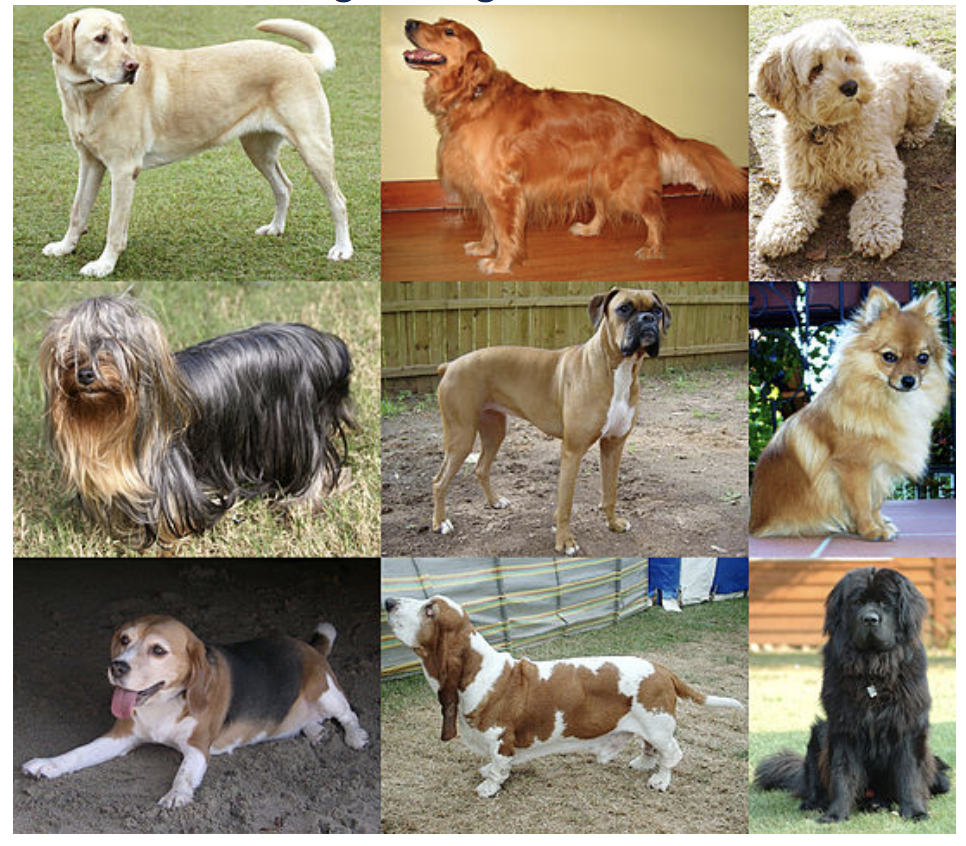
\includegraphics[width=.6\linewidth]{image/dog.png}
\end{minipage}%
\begin{minipage}{.4\textwidth}
  \centering
  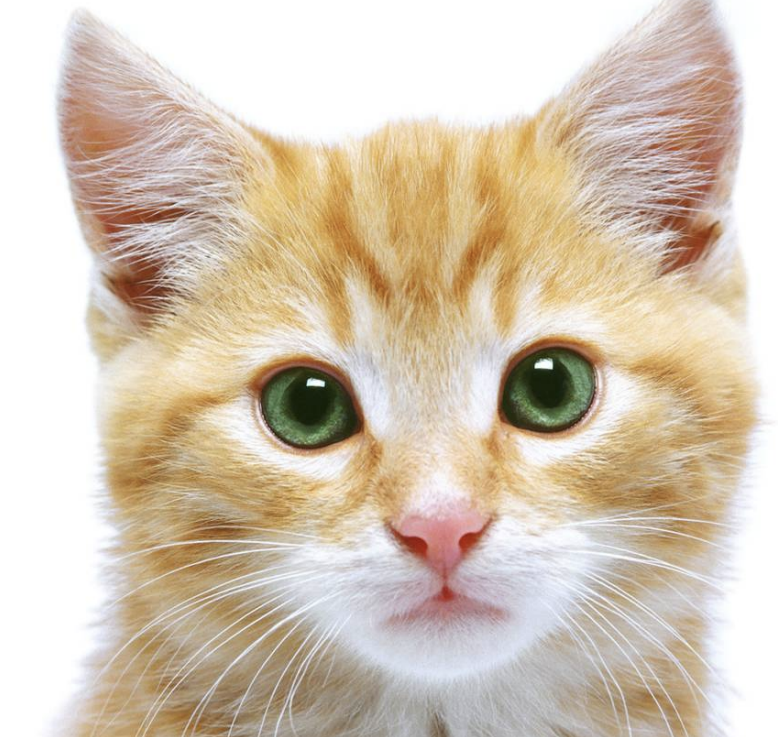
\includegraphics[width=.4\linewidth]{image/cat.png}
\end{minipage}
\end{figure}

  }
  \only<4,5,6>{
  \item     \textcolor{blue}{Instability}: A small change in the training process may produce a different result.
  % : A small change in the training process may produce a different result, and hence it is difficult to debug models or reuse parts of previous safety assessments.
  }
\only<5>{
  \begin{figure}[h]
\centering
\caption{Little variation in training procedure produce different classification rule}
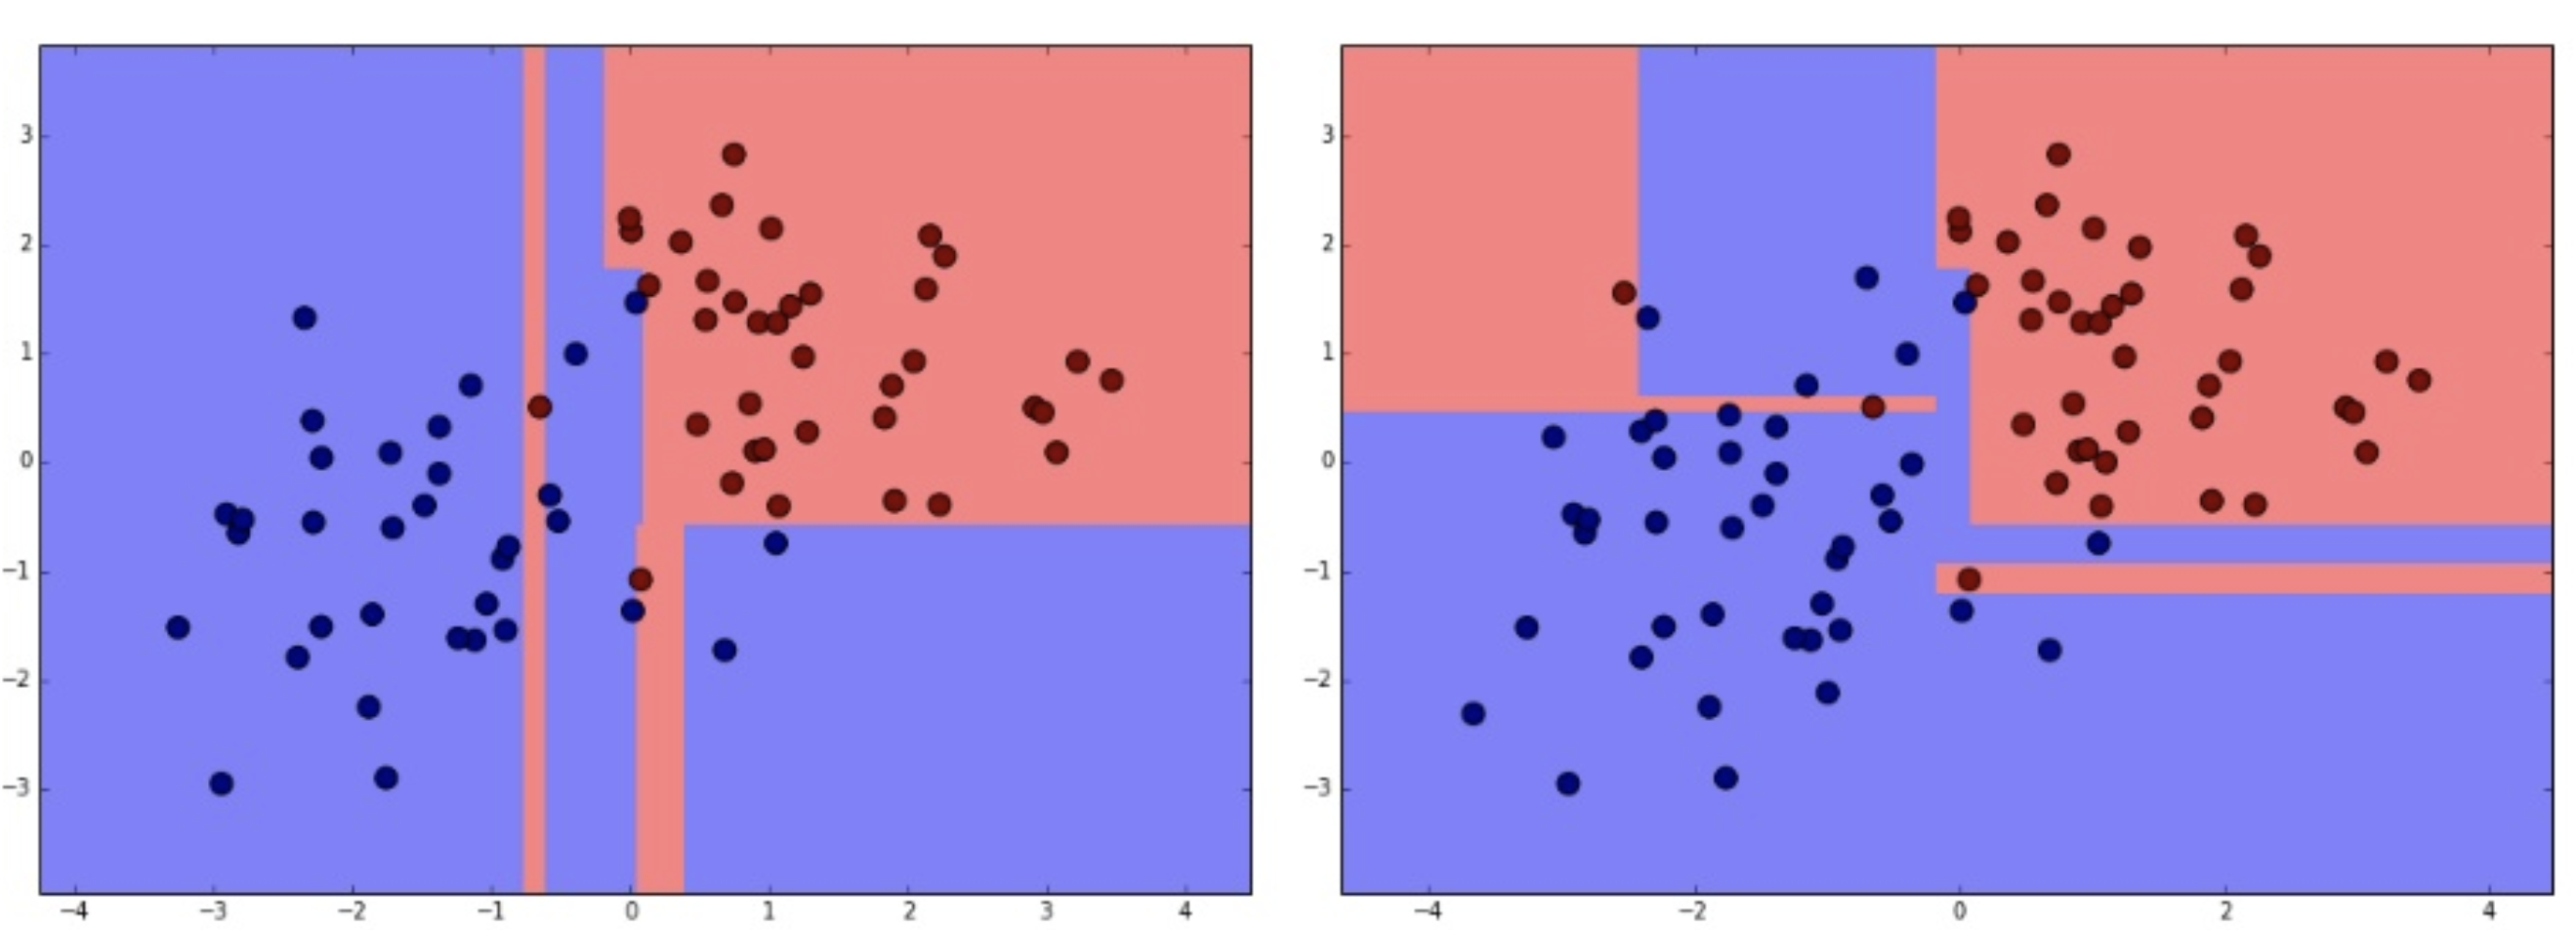
\includegraphics[scale=0.15]{image/dtvariance} 
\end{figure}
}

  \only<6>{
  \item \textcolor{blue}{Difficulty in verification}: Formal verification of ML components is a difficult, and somewhat ill-posed  problem.
  % : Formal verification of ML components is a difficult, and somewhat ill-posed, problem due to the complexity of the underlying ML algorithms and large feature spaces
}
%   \only<>{
% \item \textcolor{blue}{Incorrect specification}: The incorrect specification objective function  can result in harmful and unintended results.
% % he incorrect specification of the formal objective function, where the agent designed and deployed by a human optimises an objective function that results in harmful and unintended results
% }
\end{itemize}

\end{frame}



\section{Improve Interpretablilty and Transparency}

\begin{frame}[t]{Non-transparency}
\color{red}\rule{\linewidth}{2pt}\color{black}

Many machine learning models (e.g., deep neural network) behave mostly as black boxes.
  \begin{figure}[h]
\centering
\caption{Black Box}
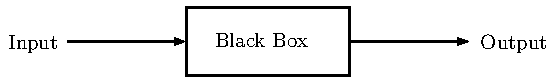
\includegraphics[scale=0.8]{image/blackbox} 
\end{figure}
\color{blue}\rule{\linewidth}{2pt}\color{black}

\justifying
Understanding the reasons behind model/prediction is, however, quite important in  \colorbox{blue!30}{assessing trust} without which if the users will not deploy/use it. 

  
\end{frame}






\begin{frame}[t]{Interpretable Models}
\color{red}\rule{\linewidth}{2pt}\color{black}

Very common model types of interpretable models are:
\begin{itemize}
\only<1>{
\item Linear regression model
\begin{align*}
  y&=w^T.\mathbf x+\epsilon\\&=w_0+\sum_{i=1}^m w_ix_i+\epsilon
\end{align*}  
}
\only<2>{
\item Decision trees.
\begin{figure}[h]
\centering
\caption{Regression Tree}
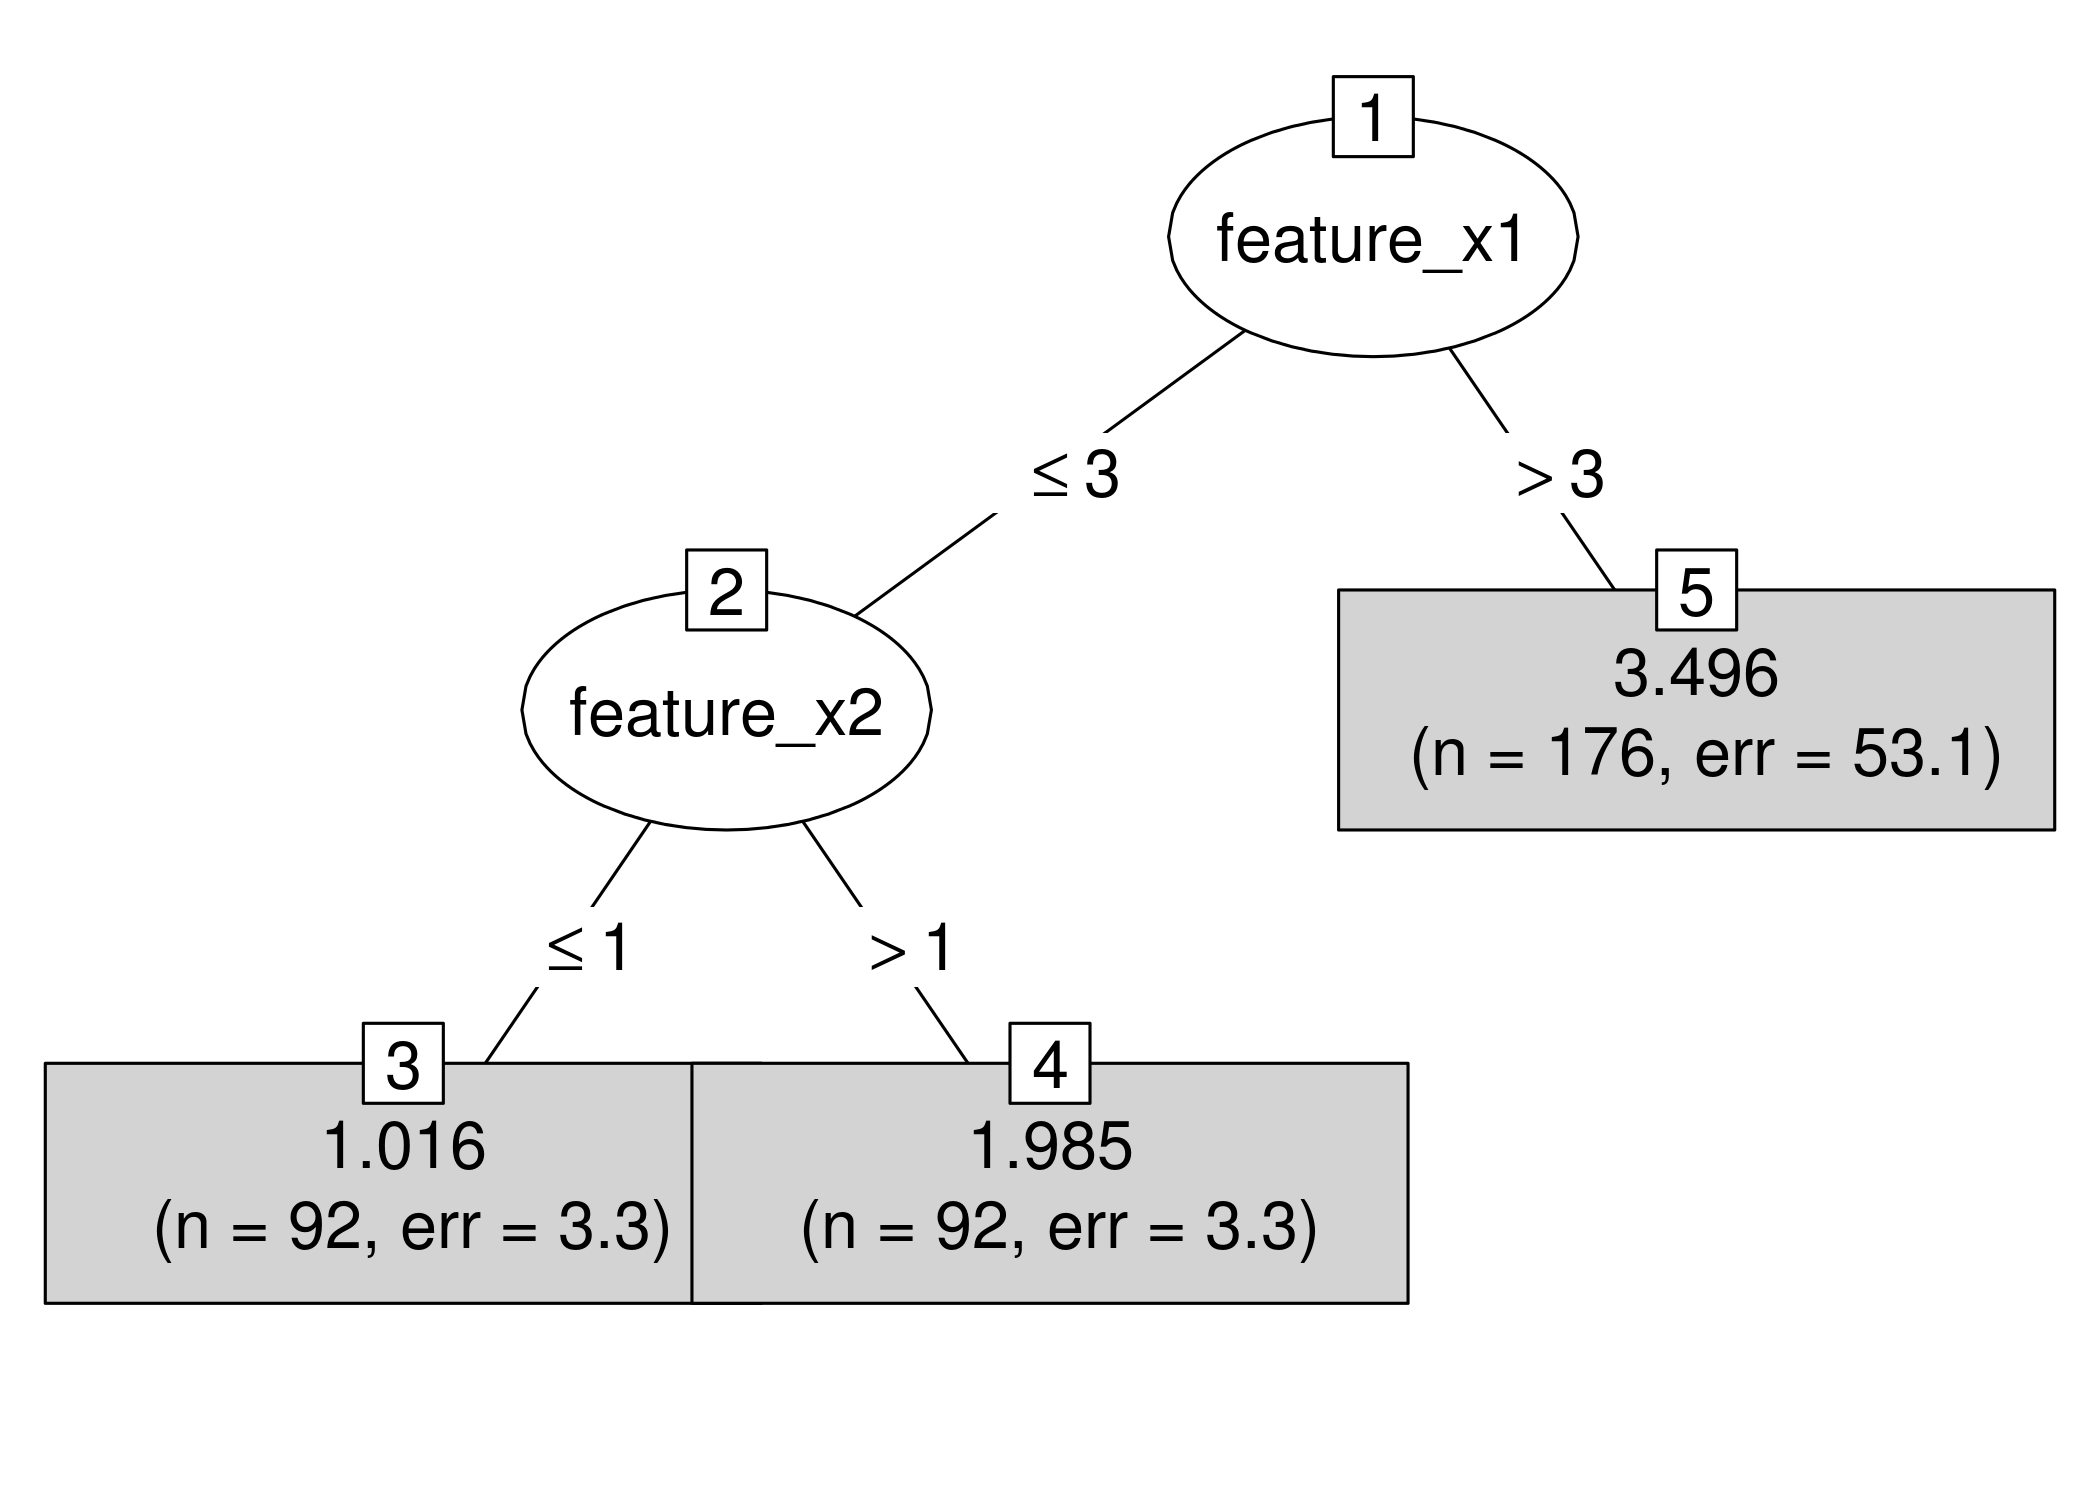
\includegraphics[scale=0.3]{image/decision_tree.png} 
\end{figure}
}
\only<3>{
\item  Decision Rules: 
\begin{semiverbatim}
If  $-3\leq x1\leq 0$ and $-2\leq x2\leq -0.5$: then $y=+1$
\end{semiverbatim} 
\begin{figure}[h]
\centering
\caption{Decision Rule}
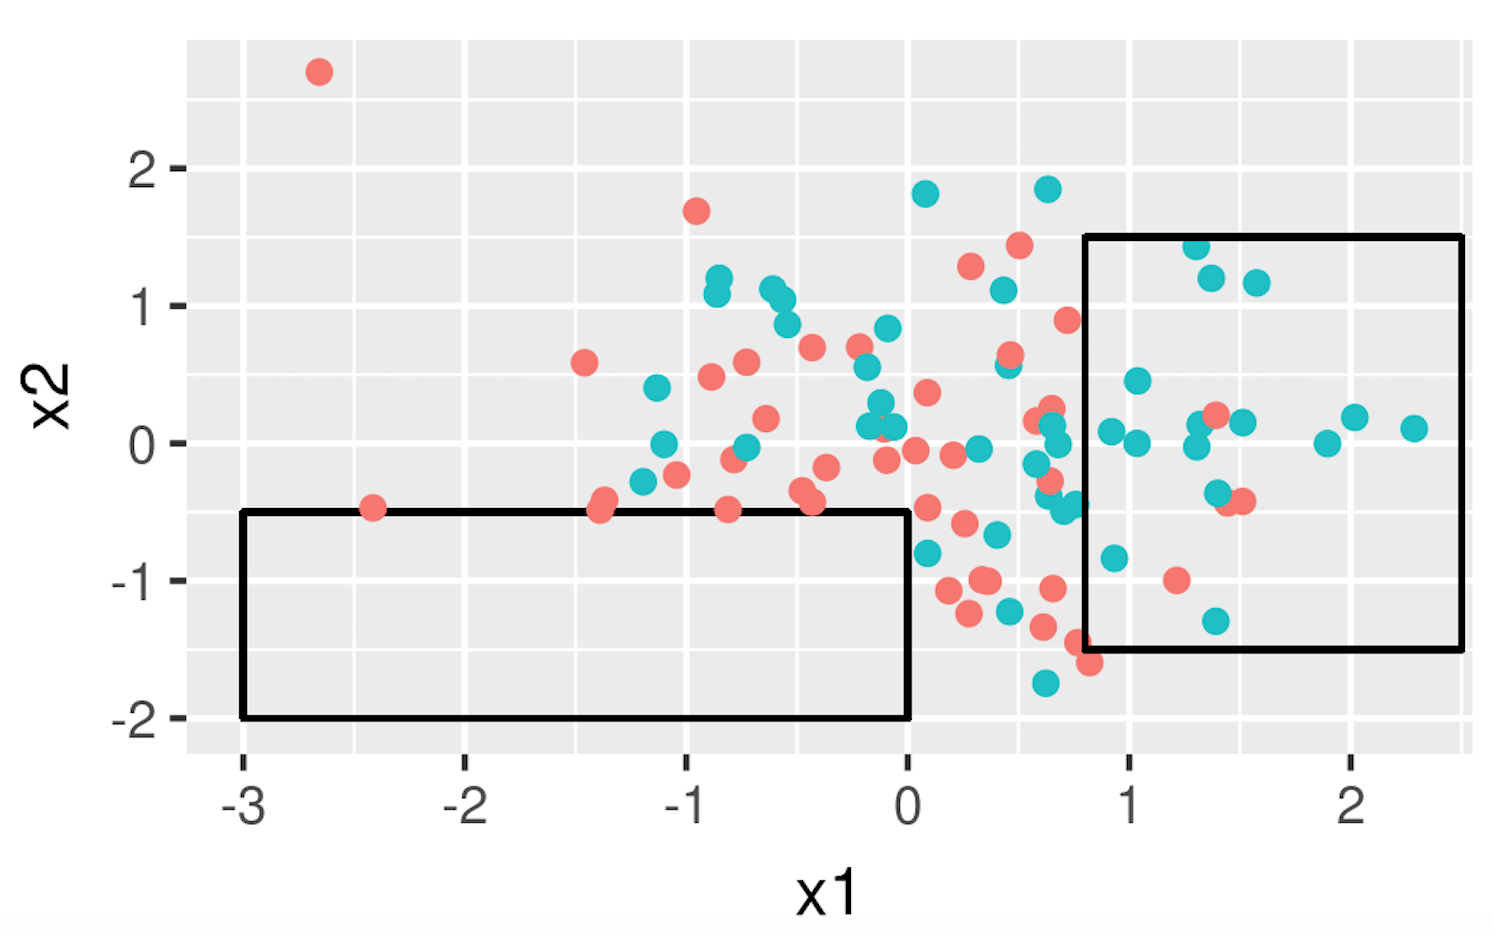
\includegraphics[scale=0.25]{image/decisionrule.png} 
\end{figure}
}
\only<4>{
\item Naive Bayes classifier
\begin{align*}
  P(y|x_1...x_d)&=\frac{P(y)P(x_1...x_d|y)}{P(x_1...x_d)}\\
&=\frac{P(y)\prod_{i=1}^d P(x_i|y)}{P(x_1...x_d)}\\
& \propto  P(y)\prod_{i=1}^d P(x_i|y)\\
\Rightarrow & y=\arg\max_y P(y)P(y)\prod_{i=1}^d P(x_i|y)
\end{align*}
 
}
\only<5>{
\item  k-Nearest Neighbors
\begin{figure}[h]
\centering
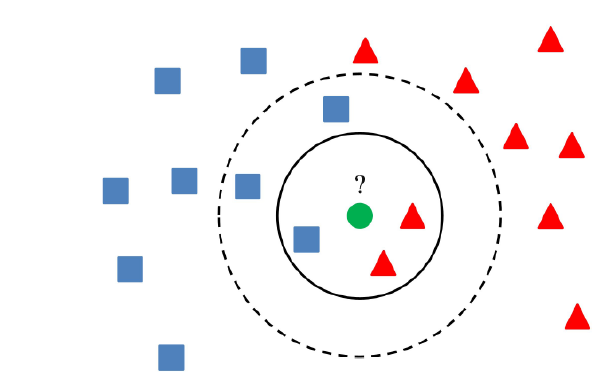
\includegraphics[scale=0.25]{image/knn.png} 
\caption{KNN (Source:wikipedia) }
\end{figure}
}

\end{itemize}




\end{frame}


\begin{frame}[t]{Explanation the Prediction}

\color{red}\rule{\linewidth}{2pt}\color{black}

\justifying
\only<1>{
Explain the prediction of a classifier by approximating it locally with an interpretable model~\cite{lime}.

\begin{figure}[h]
\centering
\caption{The black-box model's complex decision represented by the blue/pink background is approximated locally by a linear model~\cite{lime}.}
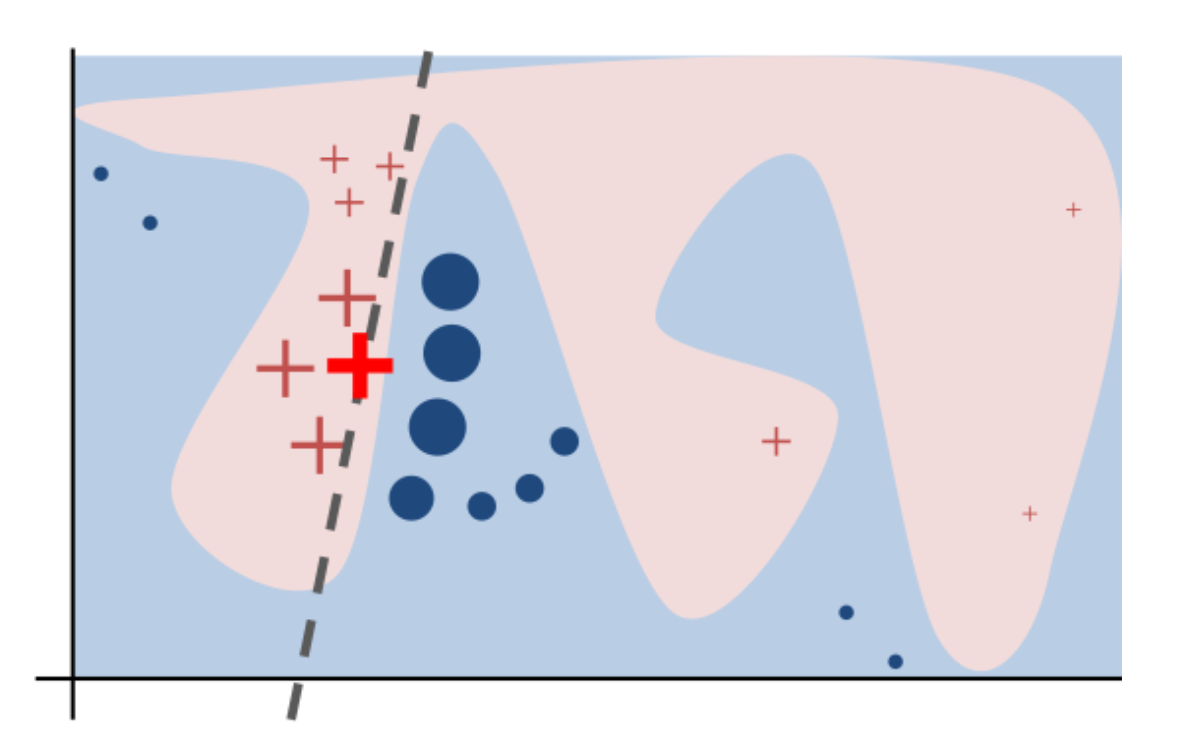
\includegraphics[scale=0.3]{image/lime2.png} 
\end{figure}
}
\only<2>{
With the explanation of a prediction, a doctor can make an informed decision about whether to trust the model's prediction.
\begin{figure}[h]
\centering
\caption{Explaining individual predictions~\cite{lime}}
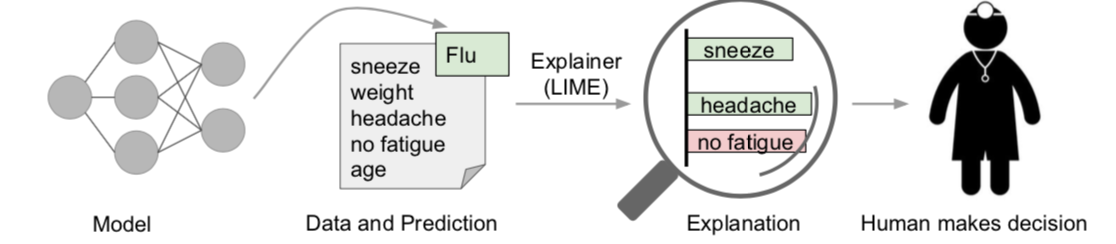
\includegraphics[scale=0.45]{image/lime.png} 
\end{figure}

}
\end{frame}




\begin{frame}[t]{Global Surrogate Models}


A global surrogate model is an interpretable model that is trained to approximate a black box model

\color{red}\rule{\linewidth}{2pt} \color{black}
\only<1>{
How well the surrogate \colorbox{blue!30}{replicates} the black box model?

\[\mbox{Metric:}1-\frac{\sum_{i=1}^n (\hat y^*_i-\hat y_i)^2}{\sum_{i=1}^n( \hat y^*_i-\bar {\hat{ y_i}})}\]
where $\hat y^*_i$  and  $\hat y_i$  is the prediction of the surrogate model and respectively  of the black box model.
}


\only<2>{
\vspace{-10mm}
\begin{figure}[h]
\centering
\caption{Linear Surrogate Model}
\includegraphics[scale=0.65]{image/surrogate} 
\end{figure}
}


\end{frame}



\section{Safe Fail}


\begin{frame}[t]{Learning to Reject}
\color{red}\rule{\linewidth}{2pt} \color{black}

\justifying
A technique used in machine learning when predictions cannot be given confidently is the  \colorbox{blue!30}{reject option}~\cite{reject}.

\[
f(x_i)=\mbox{rejection if }g(f,x_i)\leq \sigma
\]
where $g(f,x_i)$ measures the confidence level of  function f's  prediction for  $x_i$, and $\sigma$ is a threshold.

\color{blue}\rule{\linewidth}{2pt} \color{black}

\visible<2>{

When the model selects the reject option,   \colorbox{blue!30}{a human operator} can intervene and provide a manual prediction.
}
\end{frame}

\begin{frame}[t]{Confidence: Distance from Decision Boundary}

\justifying

In classification problems, classifier  implicitly assumes  that distance from the decision boundary is inversely related to confidence~\cite{errorbound}. 


 \begin{columns}[T] % align columns
\begin{column}[t]{.6\textwidth}
\color{red}\rule{\linewidth}{2pt} \color{black}

\vspace{-5mm}
\only<1,2>{
\begin{figure}[h]
\centering
\caption{Decision Boundary}
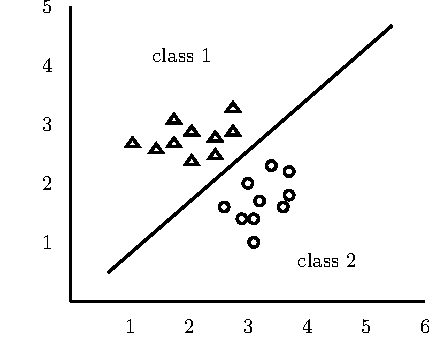
\includegraphics[scale=0.6]{image/decisionboundary} 
\end{figure}
}

\end{column}%

\begin{column}[t]{.4\textwidth}
\vspace{-5mm}

\color{blue}\rule{\linewidth}{2pt} \color{black}
\vspace{-5mm}

\only<2>{
This is reasonable \emph{to some degree} because the decision boundary is located where there is a large overlap in likelihood functions.
}


\end{column}%
\end{columns}

\end{frame}





\begin{frame}[t]{Confidence: Votes}
\justifying

\color{red}\rule{\linewidth}{2pt} \color{black}

In ensemble classification,   the overall decision $\hat y$ is based on the average classification of the base classifiers  $\hat y_i(.)$, 
\[
\phi(\mathbf x)=\frac{1}{m}\sum_{i=1}^m \hat y_i(\mathbf x)
\]

\color{blue}\rule{\linewidth}{2pt} \color{black}
\visible<2>{
The reject option of ensemble binary classification  is based on the   \colorbox{blue!30}{votes of the base classifiers\cite{errorbound}}
 \begin{align*}
  \hat y(x)=\begin{cases}-1~\mbox{ if  }\phi(\mathbf x)\leq t_1\\\mbox{reject, if }\phi( x)\in(t_1,t_2)\\1~\mbox{ if  }\phi(x)\geq t_2\end{cases}
\end{align*}

}

\end{frame}

\begin{frame}[t]{Confidence: Softmax Output}
\justifying

\color{red}\rule{\linewidth}{2pt} \color{black}

\only<1,2>{
In neural network, predictive probabilities obtained at the end of the softmax output are often erroneously interpreted as model confidence~\cite{nntogp}. 
\[
 P(y=j|\mathbf {x})=\frac { e^{\mathbf {x}^{\mathsf T} \mathbf w_j}}{
 \sum _{k=1}^{K}   e^{\mathbf x ^{\mathsf T}\mathbf w_k}}
\]
}

\color{blue}\rule{\linewidth}{2pt} \color{black}


\only<2>{
However, a model can be uncertain in its predictions even with a high softmax output~\cite{nntogp}.
}



\end{frame}




\begin{frame}[t]{Prediction Uncertainty: Gaussian Process}
A Gaussian process defines a distribution over functions $p(f)$  where $f$ is a function mapping some input space $\mathcal X\rightarrow \mathbb R$.
\only<1>
{\[ p(\mathbf f)\sim \mathcal N(0,\Sigma)=(\frac{1}{2\pi |\Sigma|})^{D/2}\exp (-1/2 \mathbf f^T \Sigma^{-1}\mathbf f)\]
}
\only<2>{


 \begin{columns}[T] % align columns
\begin{column}[t]{.65\textwidth}
\color{red}\rule{\linewidth}{2pt} \color{black}
\vspace{-5mm}

\begin{figure}[h]
\centering
\caption{One-dimensional Regression}
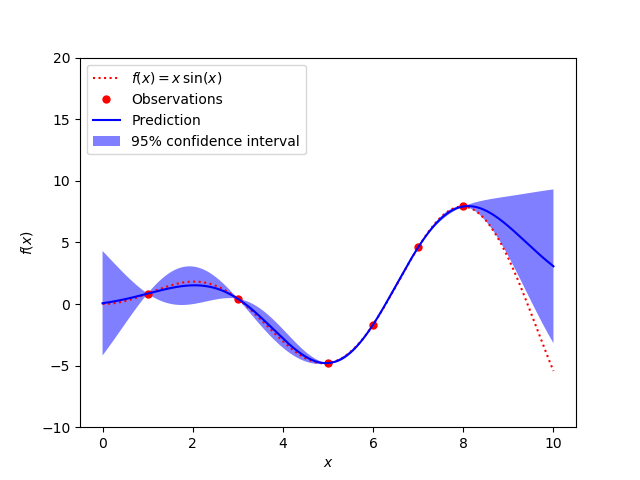
\includegraphics[scale=0.35]{image/gp1.png} 
\end{figure}
\end{column}%

\begin{column}[t]{.35\textwidth}
\vspace{-5mm}

\color{blue}\rule{\linewidth}{2pt} \color{black}

Prediction for input $\mathbf x$ with \colorbox{blue!30}{larger standard} \colorbox{blue!30}{deviation}  implicates \colorbox{blue!30}{lower confidence}. 

Thus, we can reject to predict for input input $\mathbf x$ with larger standard deviation.


\end{column}%
\end{columns}

}


\end{frame}



\begin{frame}[t]{Prediction Uncertainty: Bayesian Neural Network} 
\justifying
\color{red}\rule{\linewidth}{2pt} \color{black}
A Bayesian neural network is a neural network with a prior distribution on its weights~\cite{bnn12}, e.g., 
\[
p( \mathbf w)\sim \mathcal N(0, \sigma^2 I)
\]

\only<1>
{
\begin{figure}[h]
\centering
\caption{Prior distribution on weight~\cite{bnn12}}
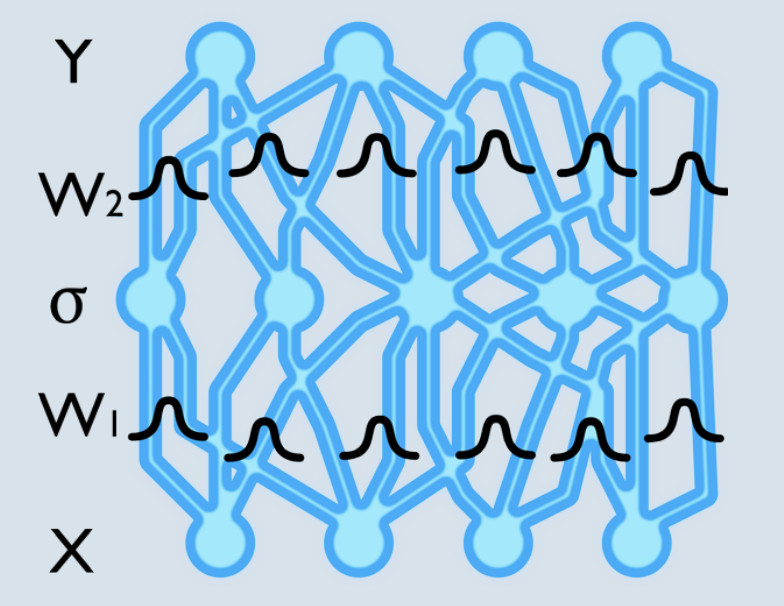
\includegraphics[scale=0.35]{image/prior.png} 
\end{figure}
}

\only<2,3>{
posterior: 
\[
P(\mathbf w|Y,X) \propto P(Y|\mathbf w,X)p(\mathbf w)
\]
}
\only<3>{
Inference:
\[
p(\mathbf y_*|\mathbf x_*,X,Y)=\int p(\mathbf y_*|\mathbf x_*,\mathbf w)p(\mathbf w|X,Y)d_{\mathbf w}
\]
}

\end{frame}


\begin{frame}[t]{Prediction with Confidence Intervals: Conformal Prediction} 
\justifying
The conform prediction~\cite{conform} gives us valid  bounds $[f(\mathbf x)-\epsilon_1,f(\mathbf x)+\epsilon_2]$ for any model such that the prediction region contains the true output with probability $\alpha$.

\begin{figure}[h]
\centering
\caption{The Bound with $95\%$ Confidence}
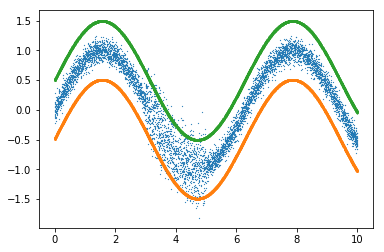
\includegraphics[scale=0.4]{image/conformal.png} 
\end{figure}

\end{frame}


\begin{frame}[t]{Reject Unmodeled Scenario} 
\justifying

It is not impossible for ML  to model everything. Thus, if the model recognize that  instance is from the input space that is not well trained, it could reject to predict.
\only<1>{
\begin{figure}[h]
\centering
\caption{Wrong Decision Boundary due to Lack of Data}
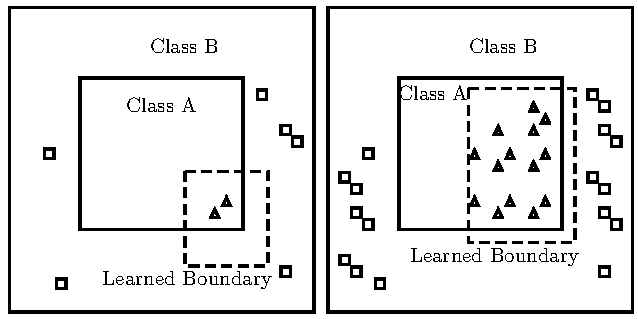
\includegraphics[scale=0.7]{image/density} 
\end{figure}
}
\only<2>{
\begin{figure}[h]
\centering
\caption{Region with Low-confidence}
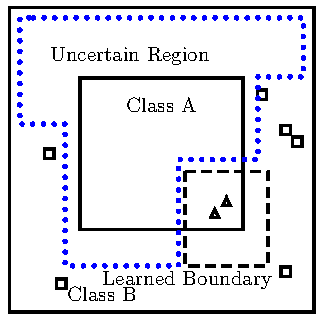
\includegraphics[scale=0.7]{image/uncertain} 
\end{figure}
}

\end{frame}

\section{Verification of ML}

\begin{frame}[t]{Challenges for Verified ML} 

\justifying
\color{red}\rule{\linewidth}{2pt} \color{black}
\only<1>{
The formal verification of ML components is a  \colorbox{blue!30}{difficult}, and somewhat  \colorbox{blue!30}{ill-posed} problem due to the  \colorbox{blue!30}{complexity} of the ML algorithms,  \colorbox{blue!30}{large feature spaces}~\cite{towardverify}.
}

\only<2,3,4>{
\alert{Challenges to achieving formally-verified ML-based systems:}
\begin{itemize}
\justifying
\only<2>{
\item  Environment Modeling: \\ It may be impossible even to precisely define all the variables (features) of the environment that must be modeled, let alone to model all possible behaviors of the environment.
\begin{figure}
\begin{minipage}{.5\textwidth}
  \centering
  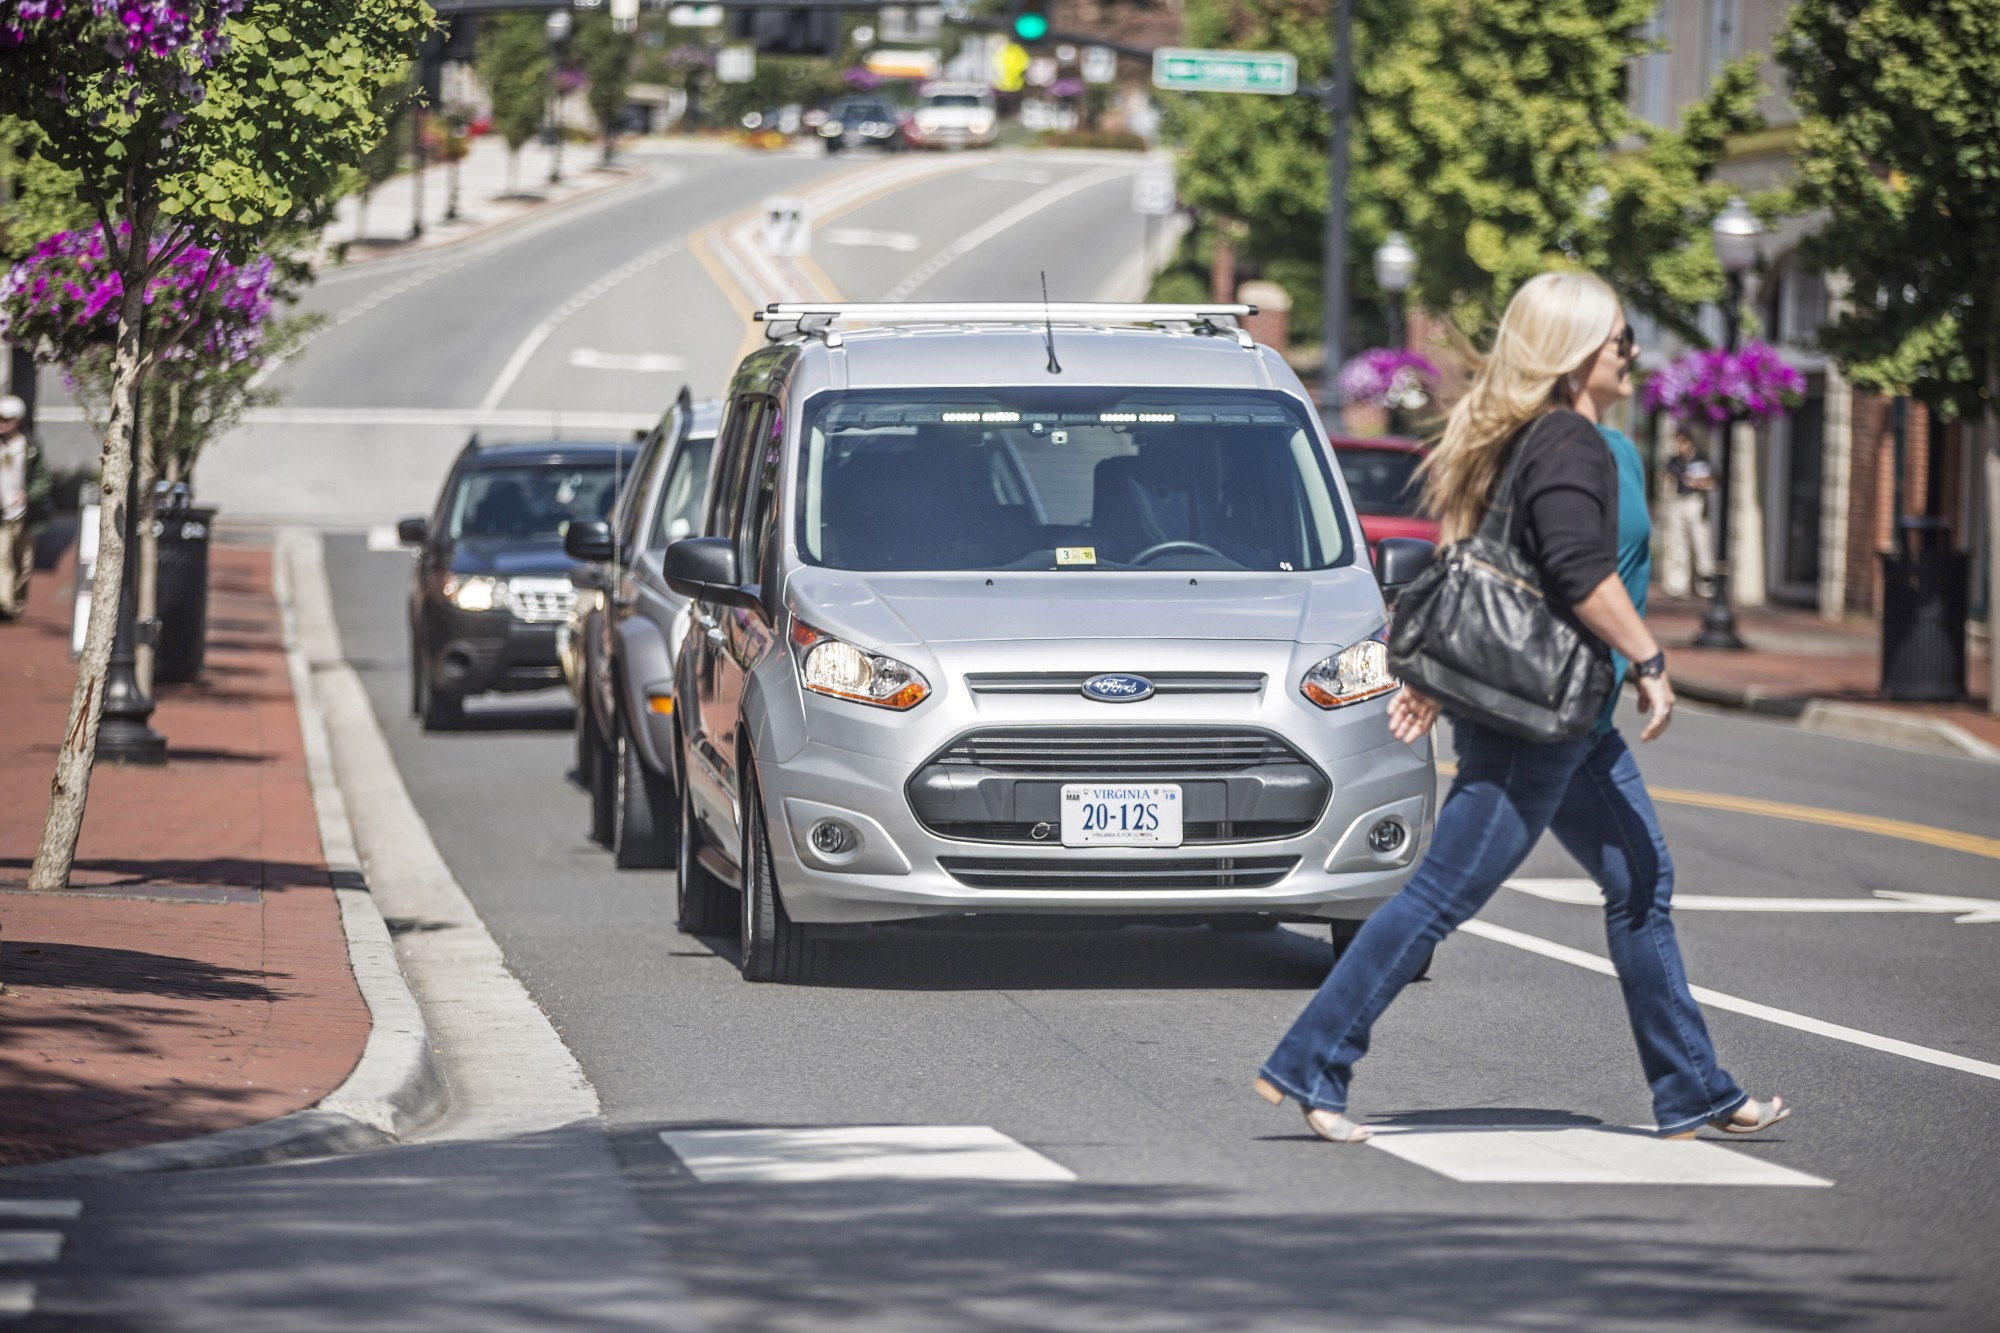
\includegraphics[width=.5\linewidth]{image/av1.jpeg}
\end{minipage}%
\begin{minipage}{.5\textwidth}
  \centering
  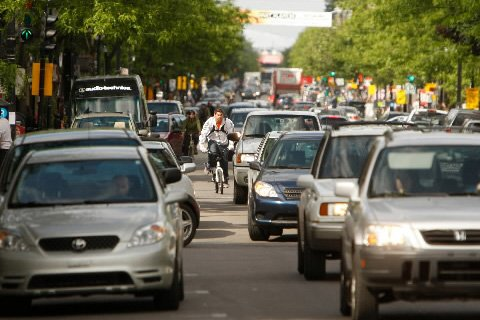
\includegraphics[width=.5\linewidth]{image/av2.jpg}
\end{minipage}
\end{figure}


}
\only<3>{
\item Specification: \\ How to specify desired and undesired properties of ML components. For example, how to  \colorbox{blue!30}{formally specify  ``a dog ''}?

\begin{figure}
\begin{minipage}{.5\textwidth}
  \centering
  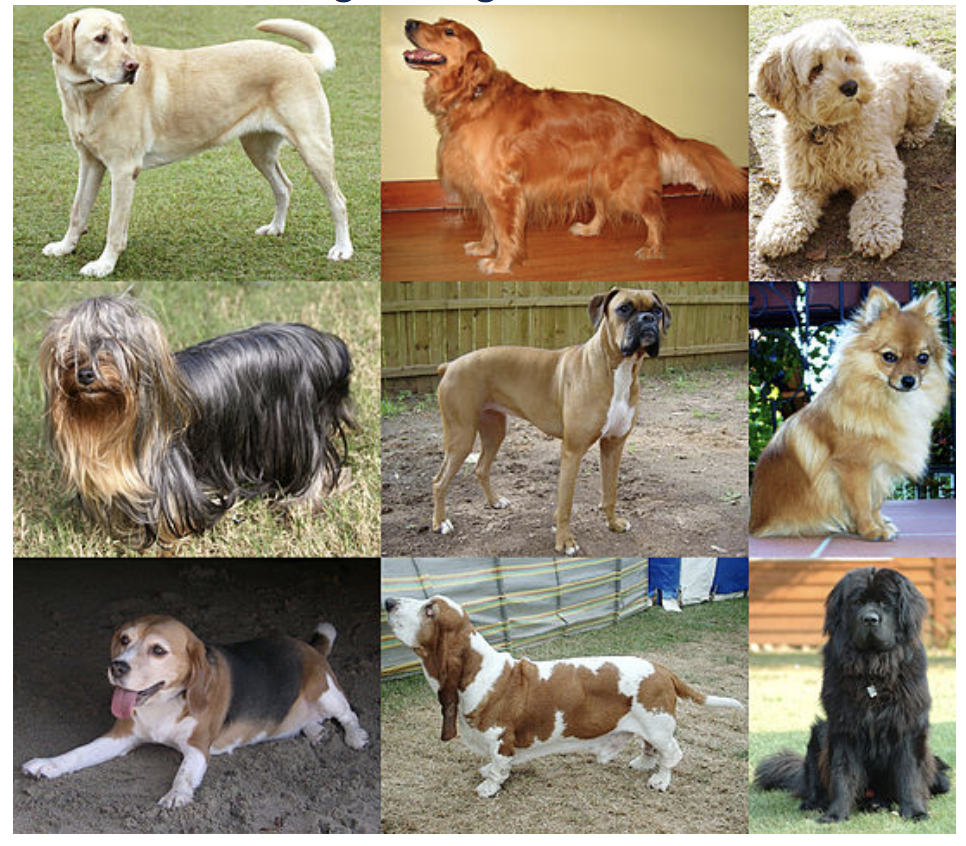
\includegraphics[width=.5\linewidth]{image/dog.png}
\end{minipage}%
\begin{minipage}{.5\textwidth}
  \centering
  
\includegraphics[width=.5\linewidth]{image/dog2.jpg}
\end{minipage}
\end{figure}

}

\only<4>{
\item   System Modeling: \\Unlike traditional applications of formal verification,   ML  based system evolves as it encounters new data and new situations. Thus, it is difficult  reuse  the previous safety verification results.

}
\end{itemize}
}
\end{frame}



\begin{frame}[t]{Go System-Level}

\justifying
\color{red}\rule{\linewidth}{2pt} \color{black}

\begin{itemize}
\item Instead of verifying  the  ML component directly, 
\item Formally specify the end-to-end behavior of the system and  verify the system containing the  ML component~\cite{abstract}.
\begin{figure}[h]
\centering
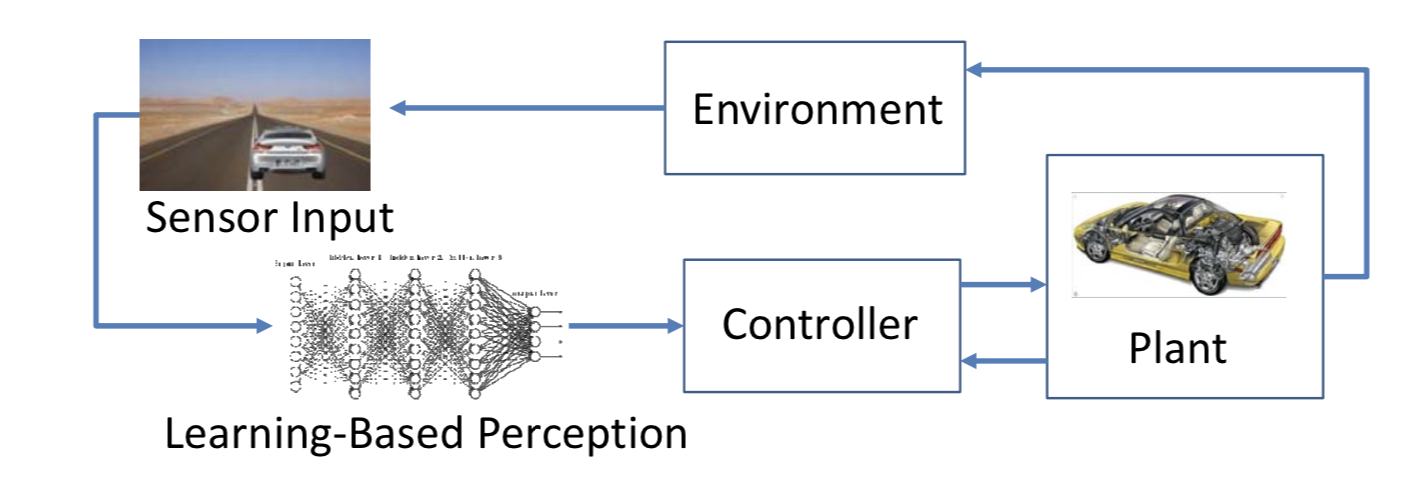
\includegraphics[scale=0.25]{image/false.png} 
\end{figure}
\end{itemize}
\only<2>{
Specification: Always (dist(ego vehicle, env object) $>\Delta$)
}
\end{frame}





\begin{frame}[t]{Approximate Model in Abstract Space} 
\justifying


 \begin{columns}[T] % align columns
\begin{column}[t]{.55\textwidth}
\color{red}\rule{\linewidth}{2pt} \color{black}
Abstract Feature Space: Instead of the high-dimensional input space,   explore   \colorbox{blue!30}{realistic and meaningful} simplification modifications~\cite{abstract}.

\begin{figure}[h]
\centering
\caption{The abstract space A with the three dimensions}
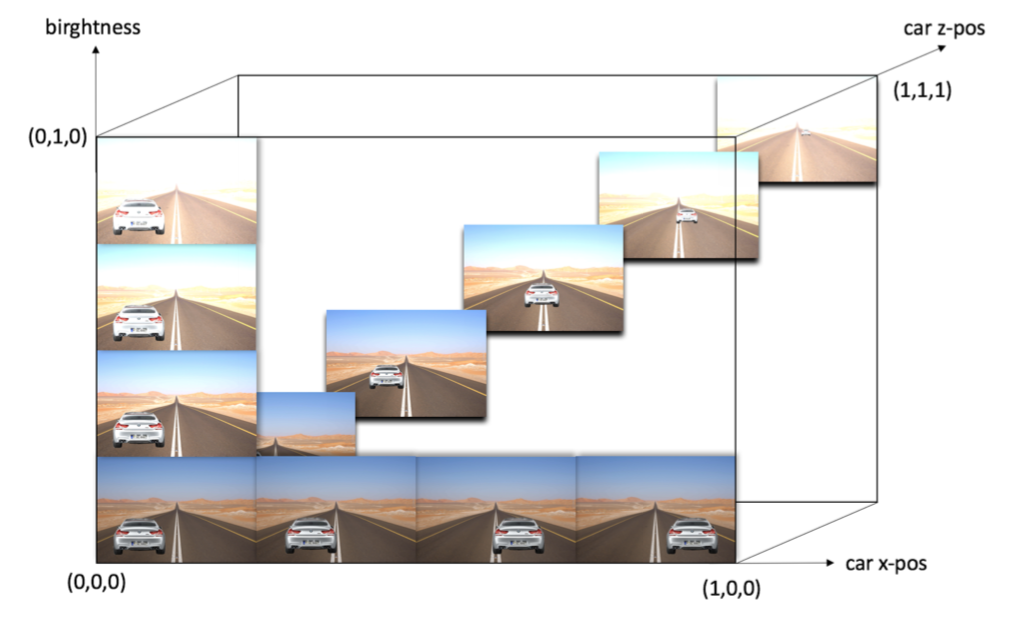
\includegraphics[scale=0.25]{image/abstract} 
\end{figure}

\end{column}%

\begin{column}[t]{.45\textwidth}
\vspace{-5mm}

\color{blue}\rule{\linewidth}{2pt} \color{black}
\vspace{-5mm}
\visible<2>{
\justifying

A simpler approximate function $\hat f $ of origin model $f$ on the abstract domain is analyzed. 
	
\begin{figure}[h]
\centering
\caption{Misclassifying Elements}
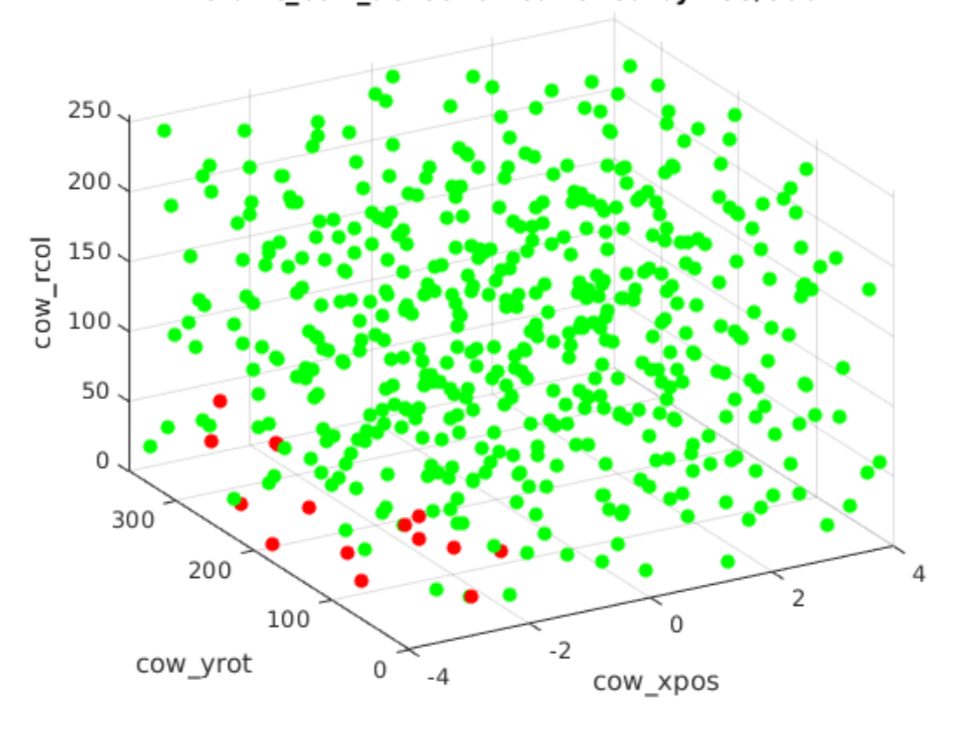
\includegraphics[scale=0.25]{image/misclassify} 
\end{figure}
}


\end{column}%
\end{columns}
\end{frame}




\begin{frame}[t]{Reduce the Problem}

\begin{itemize}
\only<1>{
	\item Reduce the input set $\mathcal X$ of n dimension into a finite number of regularized subregions. For example, partition an input set  into hyper-rectangles~\cite{reduce}.
\[
\mathcal P_i\leftarrow \mathcal I_{1,m_1}\times   \mathcal I_{2,m_2}\times \ldots \times \mathcal I_{n,m_n}
\]
where $I_{i,m_i}=[\eta_{m_i-1},\eta_{m_i}]$}
\only<2>{
\item 
For each hyper-rectangle input set, over-approximated the  output set  by a hyper-rectangle  $[\underline{\phi}_j,\bar \phi_j]$
\begin{figure}[h]
\centering
\caption{Blue rectangles: the over-approximated
output set, red spots: 5000 random outputs located in the estimated output set~\cite{reduce}}
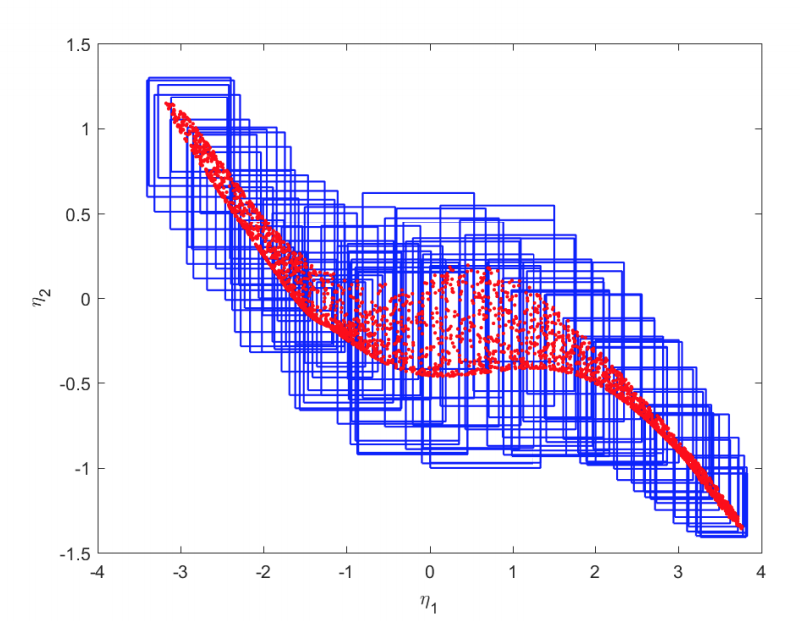
\includegraphics[scale=0.35]{image/range} 
\end{figure}

}
\end{itemize}



\end{frame}





\renewcommand{\refname}{~}
\begin{thebibliography}{1}

\bibitem{health}http://mlcenter.postech.ac.kr/healthcare
\vspace{2mm}


\bibitem{surgery}https://www.wired.com/2015/03/google-robot-surgery/
\vspace{2mm}

\bibitem{lime} Ribeiro, Marco Tulio, Sameer Singh, and Carlos Guestrin. Why should i trust you?: Explaining the predictions of any classifier. Proceedings of the 22nd ACM SIGKDD International Conference on Knowledge Discovery and Data Mining. ACM, 2016.
\vspace{2mm}

\bibitem{reject} Bartlett P L, Wegkamp M H. Classification with a reject option using a hinge loss[J]. Journal of Machine Learning Research, 2008, 9(Aug): 1823-1840.

\bibitem{Amodei} Amodei, Dario, Chris Olah, Jacob Steinhardt, Paul Christiano, John Schulman, and Dan Mane. 2016. Concrete Problems in AI Safety.

\bibitem{Bostrom} Bostrom, N., Dafoe, A., and Flynn, C. 2016. Policy Desiderata in the Development of Machine Superintelligence

\bibitem{errorbound} K. R. Varshney, R. J. Prenger, T. L. Marlatt, B. Y. Chen, and W. G. Hanley, Practical ensemble classification error bounds for different operating points, IEEE Transactions on Knowledge and Data Engineering, vol. 25, no. 11, pp. 2590-2601, Nov. 2013.
\bibitem{conform} Vovk V, Gammerman A, Shafer G. Conformal prediction[M]. Springer US, 2005

\bibitem{towardverify}  S. A. Seshia, D. Sadigh, and S. S. Sastry. Towards verified artificial intelligence. CoRR, abs/1606.08514, 2016.
 
\bibitem{abstract} Tommaso Dreossi, Alexandre Donze,  Sanjit A. Seshia, Compositional Falsification of Cyber-Physical Systems with Machine Learning Components, Preprint/

\bibitem{reduce} Weiming Xiang and Taylor T. Johnson, Reachability Analysis and Safety Verification for Neural  Network Control Systems,Preprint.

\bibitem{nntogp} Gal Y, Ghahramani Z. Dropout as a Bayesian approximation: Representing model uncertainty in deep learning[C]//international conference on machine learning. 2016: 1050-1059.
 
\bibitem{bnn12} Neal, R. M. (2012). Bayesian learning for neural networks (Vol. 118). Springer Science \& Business Media.



\end{thebibliography}

\end{document}